\documentclass[aspectratio=169]{beamer}
\useoutertheme[progressbar=frametitle]{metropolis}
\useinnertheme{metropolis}
\definecolor{nabgray}{rgb}{0.6,0.59,0.61}
\usecolortheme[named=nabgray]{structure}
\usepackage{tikz}
\usepackage[utf8]{inputenc}
\usepackage[spanish]{babel}
\usepackage{fontspec}
\setmonofont{JetBrains Mono}
\setmainfont{Roboto}
\setsansfont{Roboto}

\usepackage{smartdiagram}
\usepackage{qtree}
\usepackage{verbatim}
\usepackage{svg}
\usepackage{graphicx}
\usepackage{color}
\definecolor{lightgray}{rgb}{0.95, 0.95, 0.95}
\definecolor{darkgray}{rgb}{0.4, 0.4, 0.4}
\definecolor{ocherCode}{rgb}{1, 0.5, 0} % #FF7F00 -> rgb(239, 169, 0)
\definecolor{blueCode}{rgb}{0, 0, 0.93} % #0000EE -> rgb(0, 0, 238)
\definecolor{greenCode}{rgb}{0, 0.6, 0} % #009900 -> rgb(0, 153, 0)

\usepackage{upquote}
\usepackage{listings}
\lstset{language=java,
    otherkeywords={var,record},
    % Basic design
    backgroundcolor=\color{lightgray},
    basicstyle={\small\ttfamily},
    frame=l,
    keywordstyle=\footnotesize\color{blue},
    escapeinside={<@}{@>},
    breaklines=true,
    % Line numbers
    xleftmargin={0.75cm},
    numbers=left,
    stepnumber=1,
    firstnumber=1,
    numberfirstline=true
    % Code design
    identifierstyle=\color{black},
    keywordstyle=\color{ocherCode}\bfseries,
    ndkeywordstyle=\color{greenCode}\bfseries,
    stringstyle=\color{ocherCode}\ttfamily,
    commentstyle=\color{darkgray}\ttfamily,
    tabsize=2,
    showtabs=true,
    showspaces=false,
    showstringspaces=false,
    extendedchars=true,
    breaklines=true
}

\lstdefinelanguage{bash}{
    basicstyle=\ttfamily,
    showstringspaces=false,
    commentstyle=\color{red},
    keywordstyle=\color{blue},
    numbers=right,
    xleftmargin={0.25cm}
}

\usebackgroundtemplate
{
    
\includegraphics[width=\paperwidth]{Images/fondo}%
}


\title{Seguridad de aplicaciones Jakarta EE/MicroProfile con OWASP Top 10}
\author{Víctor Orozco - @tuxtor}
\institute{Academik}
\date{\today}

\begin{document}


{
    \usebackgroundtemplate{
\includegraphics[width=\paperwidth]{Images/portada}}
    \setbeamercolor{frametitle}{fg=red}
    \usebeamercolor[fg]{normal text}
    \frame{\titlepage}
}

\begin{frame}{Principios básicos}
	\begin{itemize}
	\item No existe un framework generico para hacer "seguridad 360"
	\item Seguridad = Balance entre necesidad de negocio/tecnología
	\item En Java hay n formas de hacer lo mismo
	\item Requerimientos -> Cifrado, firmas digitales, autenticación, autorización
	\item Herramientas
\end{itemize}
\end{frame}



{
    \usebackgroundtemplate{
\includegraphics[width=\paperwidth]{Images/separador}}
    \setbeamercolor{normal text}{fg=white}
    \setbeamercolor{frametitle}{fg=red}
    \usebeamercolor[fg]{normal text}
    \section{Seguridad en Java}
}

\begin{frame}{Infosec}
    \centering
    \smartdiagram[bubble diagram]{Seguridad,
        Confidencialidad, Integridad, Disponibilidad}
\end{frame}

\begin{frame}{Seguridad}
    \centering
    \Tree [.Seguridad JVM Lenguaje Bibliotecas ]
\end{frame}

\begin{frame}{Seguridad}
    \centering
    \Tree [.Seguridad [.JVM Escritorio Applets Invasión ] Lenguaje Bibliotecas ]
\end{frame}


\begin{frame}{Seguridad}
    \centering
    \Tree [.Seguridad JVM [.Lenguaje Tipado Punteros Scopes ] Bibliotecas ]
\end{frame}


\begin{frame}{Seguridad}
    \centering
    \Tree [.Seguridad JVM Lenguaje [.\textbf{Bibliotecas} Manual Frameworks Runtimes ] ]
\end{frame}


\begin{frame}{Bibliotecas}
    ¿Cual?
    \begin{itemize}
        \item Apache Shiro
        \item Spring Security
        \item OACC
        \item Keycloak
        \item JGuard
        \item JACC
        \item SoteriaRI
        \item MicroProfile JWT
    \end{itemize}
    . . .
\end{frame}


\begin{frame}{Tecnologias Web}
    \begin{columns}[T] % contents are top vertically aligned
        \begin{column}[T]{5cm} % each column can also be its own environment
            Render en servidor
            \begin{itemize}
                \item JSF (Icefaces, Primefaces)
                \item GWT
                \item JSP
                \item Servlets
                \item Vaadin
                \item Struts
                \item Spring MVC
            \end{itemize}
        \end{column}
        \pause
        \begin{column}[T]{5cm} % alternative top-align that's better for graphics
            Render en cliente
            \begin{itemize}
                \item Angular
                \item React
                \item Knockout (Oracle JET)
                \item Vue
            \end{itemize}
            \pause
            Servicios
            \begin{itemize}
                \item SOAP
                \item Rest
                \item RMI
            \end{itemize}
        \end{column}
    \end{columns}
\end{frame}

\begin{frame}{Tecnología}
    \begin{figure}
        \centering
        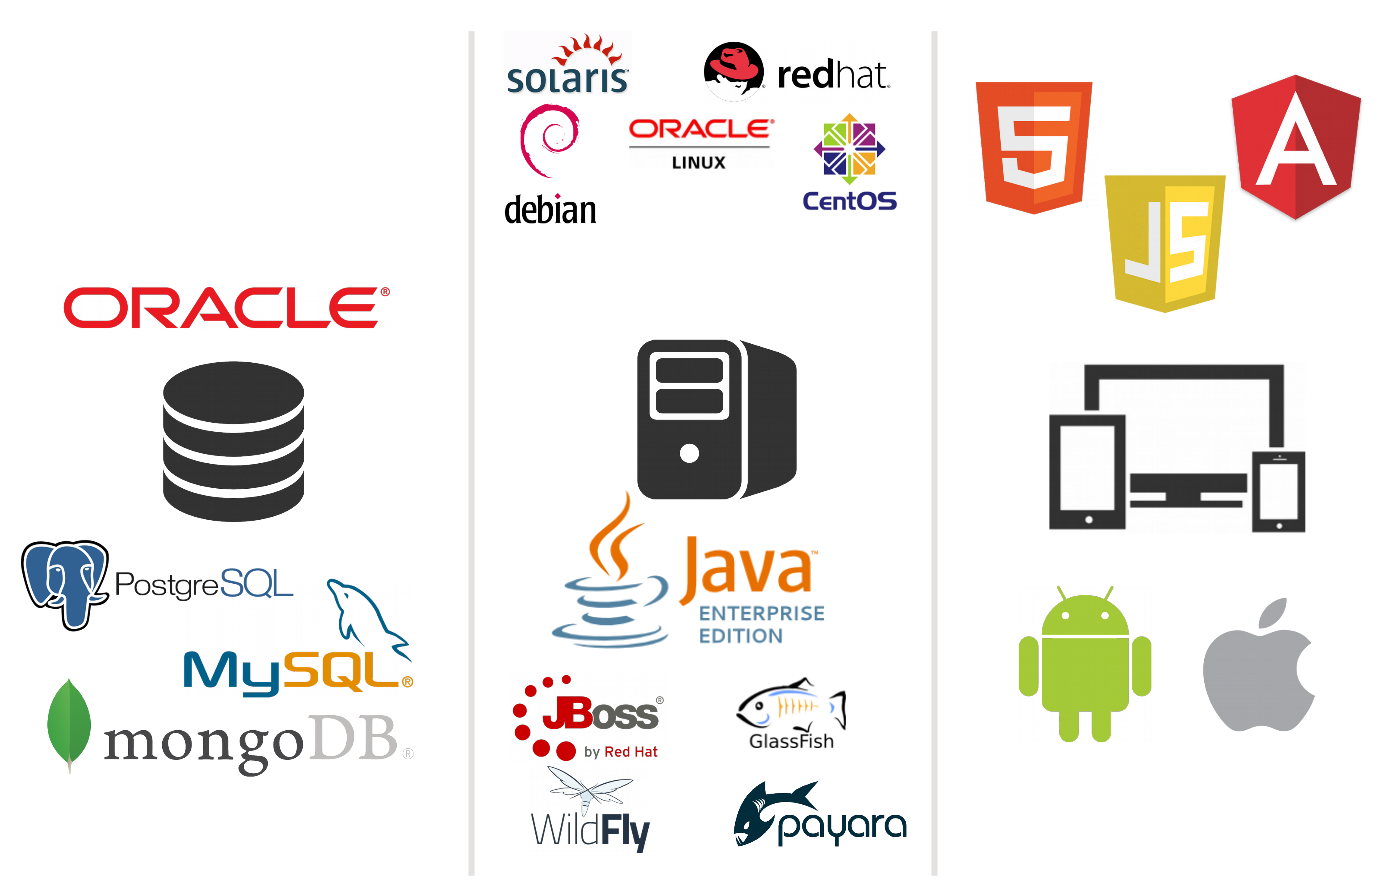
\includegraphics[width=0.8\linewidth]{Images/tecno}
    \end{figure}
\end{frame}



\begin{frame}{Jakarta EE 8}
    \begin{itemize}
        \item Mejor integración de JSF con CDI
        \item Mejor integración de JMS con CDI
        \item HTTP/2
        \item JSON-B
        \item Security
        \item JAX-RS Reactivo
    \end{itemize}
\end{frame}

\begin{frame}{JavaEE 8}
    \begin{figure}
        \centering
        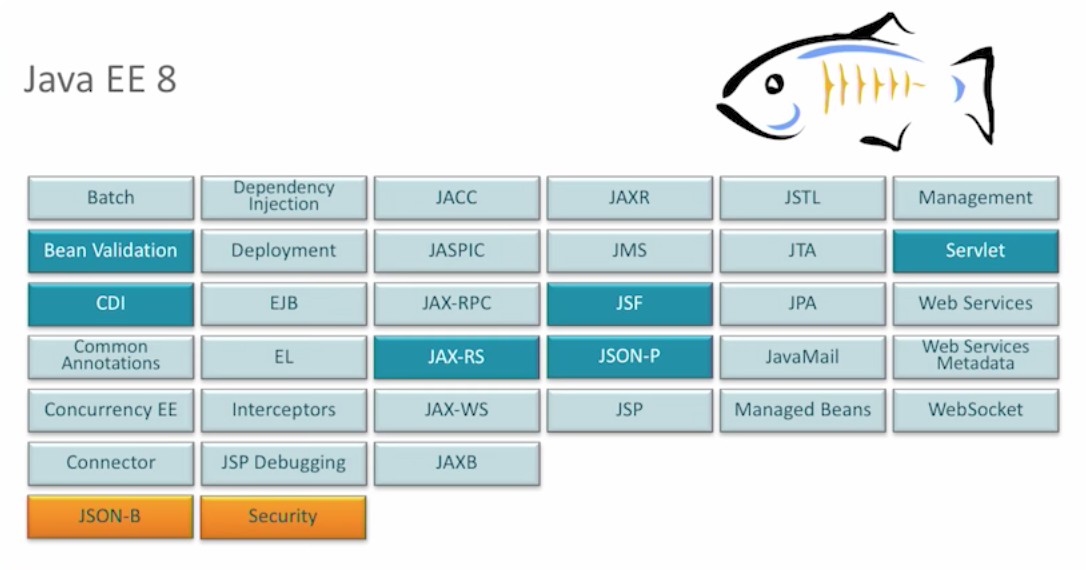
\includegraphics[width=0.9\linewidth]{Images/javaee8}
    \end{figure}
\end{frame}


\section{EE vs OWASP Top 10}

\begin{frame}{Advertencia}
    \begin{itemize}
        \item Visto en N desarrollos
        \item Un punto de inicio
        \item Informar
    \end{itemize}
\end{frame}

\begin{frame}{Top 10 OWASP}
    \begin{itemize}
        \item A1-Injection
        \item A2-Broken Authentication and Session Management
        \item A3-Sensitive Data Exposure
        \item A4-XML External Entities
        \item A5-Broken Access Control
        \item A6-Security Misconfiguration
        \item A7-Cross-Site Scripting (XSS)
        \item A8-Insecure deserialization
        \item A9-Using Components with Known Vulnerabilities
        \item A10-Insufficient Logging y Monitoring
    \end{itemize}
    \url{https://owasp.org/www-project-top-ten/}
\end{frame}

\begin{frame}{Top 10 OWASP}
    \begin{itemize}
        \item \textbf{A1-Injection}
        \item \textbf{A2-Broken Authentication and Session Management}
        \item \textbf{A3-Sensitive Data Exposure}
        \item A4-XML External Entities
        \item \textbf{A5-Broken Access Control}
        \item \textbf{A6-Security Misconfiguration}
        \item A7-Cross-Site Scripting (XSS)
        \item \textbf{A8-Insecure deserialization}
        \item \textbf{A9-Using Components with Known Vulnerabilities}
        \item A10-Insufficient Logging y Monitoring
    \end{itemize}
    \url{https://owasp.org/www-project-top-ten/}
\end{frame}


\begin{frame}{Jakarta EE - A1 - Injection}
    Problemas y causas comunes
    \begin{itemize}
        \item Concatenación de Strings en SQL
        \item Datos mal intencionados a aplicaciones
        \item Manipulación data stores
        \item Escalar privilegios
    \end{itemize}

    Sugerencias
    \begin{itemize}
        \item JAMAS y NUNCA concatenar parametros
        \item Siempre utilizar mecanismos de \texttt{sanitizing}
        \item Parchar con OWASP ESAPI
        \item JDBC y JPA soportan de serie sanitizing si no se concatena
        \item Bean Validation en parametros
    \end{itemize}
\end{frame}


\begin{frame}[fragile]{Jakarta EE - A1 - Injection}
Peligro
\begin{lstlisting}
String query = "SELECT p FROM AdmPhrase p " +
"where p.author LIKE " + author +
"and p.phrase LIKE " + phrase;

\end{lstlisting}

Mejor
\begin{lstlisting}[basicstyle=\scriptsize]
String query = "SELECT p FROM AdmPhrase p " +
    "where p.author LIKE :author " +
    "and p.phrase LIKE :phrase";

return em.createQuery(query, AdmPhrase.class)
    .setParameter("author", author)
    .setParameter("phrase", phrase)
    .getResultList();
\end{lstlisting}
\end{frame}



\begin{frame}{Jakarta EE - A2-Broken Authentication and Session Management}
    Problemas y causas comunes
    \begin{itemize}
        \item Implementación de solución manual vs frameworks
        \item Falta de políticas
        \item Entrenamiento en la plataforma
        \item Comunicación y/o autenticación via http
    \end{itemize}

    Sugerencias
    \begin{itemize}
        \item Forzar https
        \item Utilizar adecuadamente los ciclos de vida de la plataforma (singleton != stateless != statefull) y cache
        \item No implementar en base a interceptores unicamente
    \end{itemize}
\end{frame}


\begin{frame}[fragile]{Jakarta EE - A2-Broken Authentication and Session Management}
Como forzar https:

\begin{itemize}
\item API Gateway, proxy reverso, web.xml
\end{itemize}

    \begin{lstlisting}
    <security-constraint>
        <web-resource-collection>
            <web-resource-name>Viewpoint Secure URLs</web-resource-name>
            <url-pattern>/*</url-pattern>
        </web-resource-collection>
        <user-data-constraint>
            <transport-guarantee>CONFIDENTIAL</transport-guarantee>
        </user-data-constraint>
    </security-constraint>
    \end{lstlisting}
\end{frame}




\begin{frame}[fragile]{Jakarta EE - A2-Broken Authentication and Session Management}
App rest normal
\begin{lstlisting}
public class DemoinfosecRestApplication extends Application {}
\end{lstlisting}

Activar mecanismo de autenticación (MicroProfile JWT)
\begin{lstlisting}
@LoginConfig(authMethod = "MP-JWT")
@DeclareRoles({RolesEnum.Constants.MOBILE_VALUE, RolesEnum.Constants.WEB_VALUE})
public class DemoinfosecRestApplication extends Application {}
\end{lstlisting}

\end{frame}



\begin{frame}{Jakarta EE - A3-Sensitive data exposure}
    Problemas y causas comunes
    \begin{itemize}
        \item Guardar datos sin cifrar
        \item Datos con cifrado "debil", AKA cifrado propio
        \item Transmitir credenciales via http
        \item Transmisión de excepciones completas a front-end
    \end{itemize}

    Sugerencias
    \begin{itemize}
        \item Identificar con un checklist los datos sensitivos
        \item Evitar cifrado de dos vías a menos que sea necesario
        \item Evitar transmisión de llaves
        \item Verificar código auto generado (excepciones)
    \end{itemize}
\end{frame}


\begin{frame}{Jakarta EE - A5-Broken Access Control}
    Problemas y causas comunes
    \begin{itemize}
        \item Implementación de solución manual vs frameworks
        \item Falta de políticas
        \item Escalar privilegios
        \item Comunicación y/o autenticación via http
    \end{itemize}

    Sugerencias
    \begin{itemize}
        \item Forzar https
        \item Implementación RBAC de application server
        \item Implementación RBAC de framework
        \item Entender el modelo de JAAS, Spring Security, SoteriaRI y MicroProfile JWT
    \end{itemize}
\end{frame}


\begin{frame}[fragile]{Jakarta EE - A5-Broken Access Control}
Endpoint normal
\begin{lstlisting}
@GET
@Path("/{id:[0-9][0-9]*}")
public AdmPhrase findById(@PathParam("id") Long id) {
    return admPhraseRepository.findById(id);
}
\end{lstlisting}

Endpoint con RBAC
\begin{lstlisting}
@GET
@Path("/{id:[0-9][0-9]*}")
@RolesAllowed({RolesEnum.Constants.MOBILE_VALUE, RolesEnum.Constants.WEB_VALUE})
public AdmPhrase findById(@PathParam("id") Long id) {
    return admPhraseRepository.findById(id);
}
\end{lstlisting}

\end{frame}




\begin{frame}{Jakarta EE - A6-Security Misconfiguration}
    Problemas y causas comunes
    \begin{itemize}
        \item Configuración por defecto de applicaction server
        \item Configuración por defecto de SO
        \item Configuración \texttt{relajada} de capa de transporte
    \end{itemize}

    Sugerencias
    \begin{itemize}
        \item Configurar siempre el SO destino
        \item Proteger y actualizar runtime
        \item Firewall
        \item RBAC
        \item Evitar certificados autofirmados en entornos no controlados
        \item JVM tipo \texttt{server}
    \end{itemize}
\end{frame}


\begin{frame}{Jakarta EE - A8-Insecure deserialization}
    Problemas y causas comunes
    \begin{itemize}
        \item Self made frameworks
        \item No hay validación
    \end{itemize}

    Sugerencias
    \begin{itemize}
        \item Evaluar si no vale la pena utilizar un framework listo y probado
        \item Bean validation
        \item Sanitización
    \end{itemize}
\end{frame}


\begin{frame}{Jakarta EE - A9-Using components with known vulnerabilities}
    Problemas y causas comunes
    \begin{itemize}
        \item Difícil dar seguimiento a los lanzamientos
        \item Frameworks muy nuevos o muy viejos
        \item No seguir las notas del lanzamiento
    \end{itemize}

    Sugerencias
    \begin{itemize}
        \item Actualizar el app server con el calendario de lanzamiento
        \item Suscripción a mailing list/foros
        \item Servicios tipo Bintray, GitHub Security
        \item Servicios de análisis estático (Sonar)
    \end{itemize}
\end{frame}

\begin{frame}{Jakarta EE - A9-Using components with known vulnerabilities}
    \begin{figure}
        \centering
        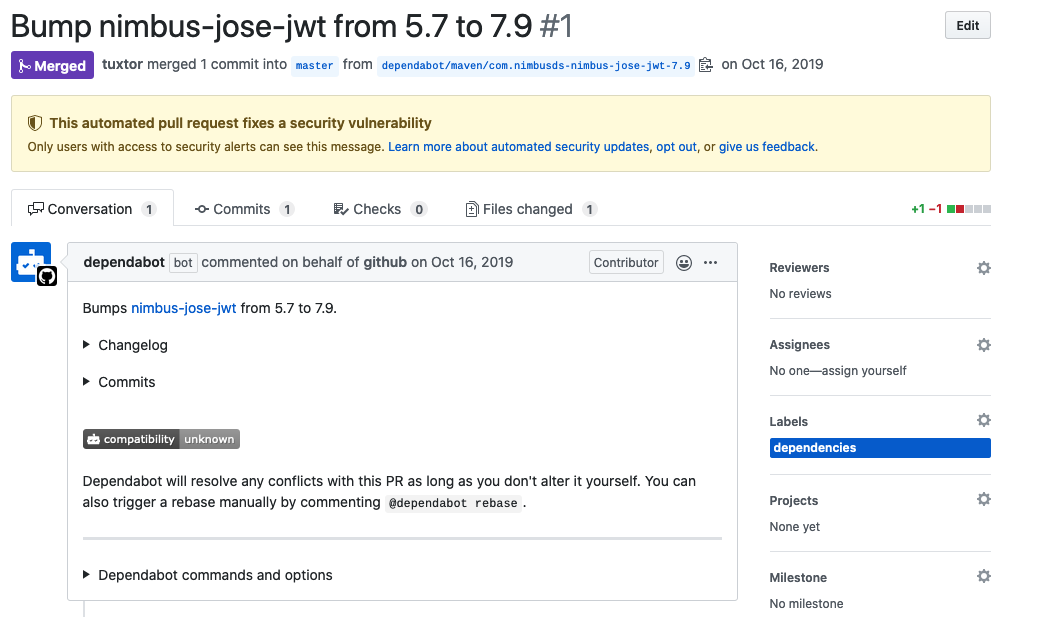
\includegraphics[width=0.9\linewidth]{Images/github}
    \end{figure}
\end{frame}

\begin{frame}{Jakarta EE - Bonus-APIs sin proteger}
    Problemas y causas comunes
    \begin{itemize}
        \item Combinación de broken auth, broken access control o security misconfiguration
        \item A veces simplemente no hay seguridad porque "a mi no me van a atacar"
        \item Especialmente grave en rich clients
    \end{itemize}

    Sugerencias
    \begin{itemize}
        \item Verificar código auto generado
        \item Programar en modo \texttt{deny all}
    \end{itemize}
\end{frame}

{
    \usebackgroundtemplate{
\includegraphics[width=\paperwidth]{Images/separador}}
    \setbeamercolor{normal text}{fg=white}
    \setbeamercolor{frametitle}{fg=red}
    \usebeamercolor[fg]{normal text}
    \section{Demo}
}

\begin{frame}{Demo Payara 5}
    \begin{figure}
        \centering
        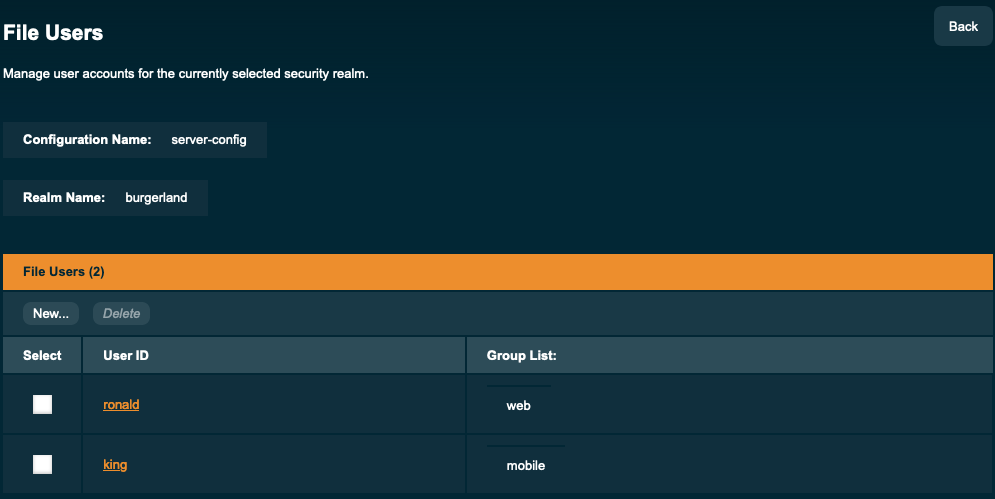
\includegraphics[width=0.9\linewidth]{Images/realms}
    \end{figure}
\end{frame}

\begin{frame}{Demo Payara 5}
    \begin{itemize}
        \item Proveedor de tokens \href{https://github.com/tuxtor/microjwt-provider/}{https://github.com/tuxtor/microjwt-provider/}
        \item API protegida \href{https://github.com/tuxtor/demoinfosec-service-b/}{https://github.com/tuxtor/demoinfosec-service-b/}
    \end{itemize}
\end{frame}



\begin{frame}{Víctor Orozco}
    \begin{columns}[T] % contents are top vertically aligned

        \begin{column}[T]{4cm} % alternative top-align that's better for graphics
            \begin{figure}
                \centering
                
\includegraphics[width=\linewidth]{Images/logos}
            \end{figure}
        \end{column}
        \begin{column}[T]{6cm} % each column can also be its own environment
            \begin{itemize}
                \item vorozco@nabenik.com
                \item \href{https://twitter.com/tuxtor}{@tuxtor}
                \item \href{http://vorozco.com}{http://vorozco.com}
                \item \href{http://tuxtor.shekalug.org}{http://tuxtor.shekalug.org}
            \end{itemize}
            \begin{center}
                
\includegraphics[width=0.1\linewidth]{Images/cclogo}
                \\
                This work is licensed under Creative Commons Attribution-NonCommercial-ShareAlike 3.0 Guatemala (CC BY-NC-SA 3.0 GT).
            \end{center}
        \end{column}
    \end{columns}
\end{frame}

{
    \usebackgroundtemplate{
\includegraphics[width=\paperwidth]{Images/final}}
    \begin{frame}
    \end{frame}
}

\end{document}

